\chapter{Caching Algorithms}
Caching algorithms are used to manage the content of a cache when dealing with a series of requests from a computer. When the cache becomes full, these algorithms decide which pieces of data to evict. The eviction policy is different for every algorithm, but the general goal is the same, to minimize the cost of cache misses as they decrease the overall performance of the system.


\section{Least Recently Used}


The Least Recently Used(LRU) algorithm has an intuitive structure and a relatively simple implementation. When choosing which item to evict from a cache, it evicts the item least recently referenced. This means that when LRU decides to evict something from the cache, it looks at the trace from the current request back to the start of the trace and chooses the item which is currently in the cache whose most recent reference is farthest from the current request. This makes LRU well-suited for applications where a small set of items are accessed together as it keeps items frequently accessed in the cache.


Figure 3.1 is a basic example of how LRU works given a simple trace. LRU functions exceptionally well on this trace, only missing on the first occurrence of an item due to the trace's tendency to request a subset of items frequently. This means that due to the lack of misses on this trace given LRU, this cache would cause a minimal performance penalty as it only misses items it hasn't seen yet. 
\begin{figure}[H]
    \centering
    \caption{LRU cache given: A,B,C,D,B,C,D}
    \label{fig:my_label}
\begin{tikzpicture}
\node[rounded corners,draw=black,label=above:LRU, minimum size=2cm] (a) at (0,0)  {
    \begin{tikzpicture}
        \node[rounded corners,draw=black,minimum size=0.8cm]{A};
    \end{tikzpicture}
    
\begin{tikzpicture}
        \node[rounded corners,draw=black,minimum size=0.8cm]{};
    \end{tikzpicture}
    
\begin{tikzpicture}
        \node[rounded corners,draw=black,minimum size=0.8cm]{};
    \end{tikzpicture}
    };
    \node[text width=3cm] at (-3, 0) 
    {Miss on A as first instance, add A to cache};

    
    \node[rounded corners,draw=black,minimum size=2cm] (b) at (0,-2.5)  {   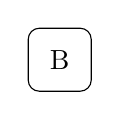
\begin{tikzpicture}
        \node[rounded corners,draw=black,minimum size=0.8cm]{B};
    \end{tikzpicture}
    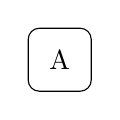
\begin{tikzpicture}
        \node[rounded corners,draw=black,minimum size=0.8cm]{A};
    \end{tikzpicture}
    
\begin{tikzpicture}
        \node[rounded corners,draw=black,minimum size=0.8cm]{};
    \end{tikzpicture}
    };
     \node[text width=3cm] at (-3,-2.5) 
    {Miss on B as first instance, add B to cache};
    
    \node[rounded corners,draw=black,minimum size=2cm] (c) at (0,-5)  {   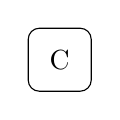
\begin{tikzpicture}
        \node[rounded corners,draw=black,minimum size=0.8cm]{C};
    \end{tikzpicture}
    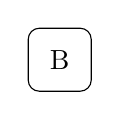
\begin{tikzpicture}
        \node[rounded corners,draw=black,minimum size=0.8cm]{B};
    \end{tikzpicture}
    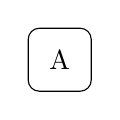
\begin{tikzpicture}
        \node[rounded corners,draw=black,minimum size=0.8cm]{A};
    \end{tikzpicture}
    };

    \node[text width=3cm] at (-3,-5) 
    {Miss on C as first instance, C added to cache};
      
    \node[rounded corners,draw=black,minimum size=2cm] (d) at (0,-7.5)  {   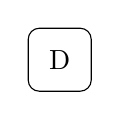
\begin{tikzpicture}
        \node[rounded corners,draw=black,minimum size=0.8cm]{D};
    \end{tikzpicture}
    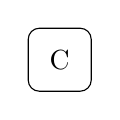
\begin{tikzpicture}
        \node[rounded corners,draw=black,minimum size=0.8cm]{C};
    \end{tikzpicture}
    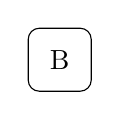
\begin{tikzpicture}
        \node[rounded corners,draw=black,minimum size=0.8cm]{B};
    \end{tikzpicture}
    };

     \node[text width=3cm] at (-3,-7.5) 
    {Miss on D as first instance, evict A since LRU};
    
    \node[rounded corners,draw=black,minimum size=2cm, below left=1 cm of d] (e) at (2.2,-8.4)  { 
    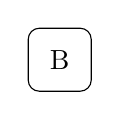
\begin{tikzpicture}
        \node[rounded corners,draw=black,minimum size=0.8cm]{B};
    \end{tikzpicture}
    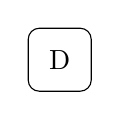
\begin{tikzpicture}
        \node[rounded corners,draw=black,minimum size=0.8cm]{D};
    \end{tikzpicture}
    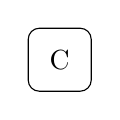
\begin{tikzpicture}
        \node[rounded corners,draw=black,minimum size=0.8cm]{C};
    \end{tikzpicture}
    };  

     \node[text width=3cm] at (-3,-10) 
    {Hit on B};

    \node[rounded corners,draw=black,minimum size=2cm, below left=1 cm of d] (f) at (2.2,-11)  { 
    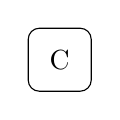
\begin{tikzpicture}
        \node[rounded corners,draw=black,minimum size=0.8cm]{C};
    \end{tikzpicture}
    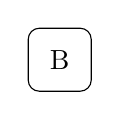
\begin{tikzpicture}
        \node[rounded corners,draw=black,minimum size=0.8cm]{B};
    \end{tikzpicture}
    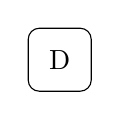
\begin{tikzpicture}
        \node[rounded corners,draw=black,minimum size=0.8cm]{D};
    \end{tikzpicture}
    };  

     \node[text width=3cm] at (-3,-12.5) 
    {Hit on C};

    \node[rounded corners,draw=black,minimum size=2cm, below left=1 cm of d] (g) at (2.2,-13.5)  { 
    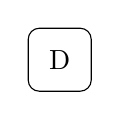
\begin{tikzpicture}
        \node[rounded corners,draw=black,minimum size=0.8cm]{D};
    \end{tikzpicture}
    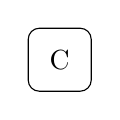
\begin{tikzpicture}
        \node[rounded corners,draw=black,minimum size=0.8cm]{C};
    \end{tikzpicture}
    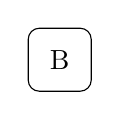
\begin{tikzpicture}
        \node[rounded corners,draw=black,minimum size=0.8cm]{B};
    \end{tikzpicture}
    };  

     \node[text width=3cm] at (-3,-15) 
    {Hit on D};

    \draw[thick,->] (a) -- (b);
    \draw[thick,->](b) -- (c);  
    \draw[thick,->](c) -- (d);  
    \draw[thick,->](d) -- (e);  
    \draw[thick,->](e) -- (f);  
    \draw[thick,->](f) -- (g);  
\end{tikzpicture}
\end{figure}



\section{Most Recently Used}
The Most Recently Used (MRU) algorithm is an algorithm that when a cache becomes full of items, evicts the most recently used item. This means that when needing to evict an item, MRU evicts the last item that was requested just before the current request. This makes MRU suited for traces where items referenced furthest in the past are more likely to be requested again than those accessed more recently.

Figure 3.2 is a basic example of how MRU works. On this trace, MRU only misses the first instance of an item as, after the first instance of an item, the cache is unlikely to see it accessed again soon, as A in this trace. 

\begin{figure}[H]
    \centering
    \caption{MRU cache given: A,B,C,D,B,D,A}
    \label{fig:my_label}
\begin{tikzpicture}
\node[rounded corners,draw=black,label=above:MRU, minimum size=2cm] (a) at (0,0)  {
    \begin{tikzpicture}
        \node[rounded corners,draw=black,minimum size=0.8cm]{A};
    \end{tikzpicture}
    
\begin{tikzpicture}
        \node[rounded corners,draw=black,minimum size=0.8cm]{};
    \end{tikzpicture}
    
\begin{tikzpicture}
        \node[rounded corners,draw=black,minimum size=0.8cm]{};
    \end{tikzpicture}
    };
    \node[text width=3cm] at (-3, 0) 
    {Miss on A as first instance, add A to cache};

    
    \node[rounded corners,draw=black,minimum size=2cm] (b) at (0,-2.5)  {   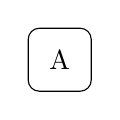
\begin{tikzpicture}
        \node[rounded corners,draw=black,minimum size=0.8cm]{A};
    \end{tikzpicture}
    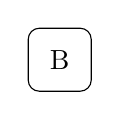
\begin{tikzpicture}
        \node[rounded corners,draw=black,minimum size=0.8cm]{B};
    \end{tikzpicture}
    
\begin{tikzpicture}
        \node[rounded corners,draw=black,minimum size=0.8cm]{};
    \end{tikzpicture}
    };
     \node[text width=3cm] at (-3,-2.5) 
    {Miss on B as first instance, add B to cache};
    
    \node[rounded corners,draw=black,minimum size=2cm] (c) at (0,-5)  {   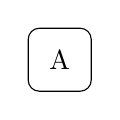
\begin{tikzpicture}
        \node[rounded corners,draw=black,minimum size=0.8cm]{A};
    \end{tikzpicture}
    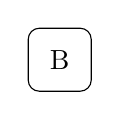
\begin{tikzpicture}
        \node[rounded corners,draw=black,minimum size=0.8cm]{B};
    \end{tikzpicture}
    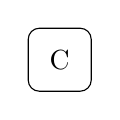
\begin{tikzpicture}
        \node[rounded corners,draw=black,minimum size=0.8cm]{C};
    \end{tikzpicture}
    };

    \node[text width=3cm] at (-3,-5) 
    {Miss on C as first instance, C added to cache};
      
    \node[rounded corners,draw=black,minimum size=2cm] (d) at (0,-7.5)  {   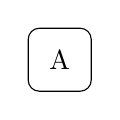
\begin{tikzpicture}
        \node[rounded corners,draw=black,minimum size=0.8cm]{A};
    \end{tikzpicture}
    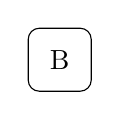
\begin{tikzpicture}
        \node[rounded corners,draw=black,minimum size=0.8cm]{B};
    \end{tikzpicture}
    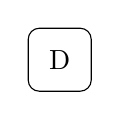
\begin{tikzpicture}
        \node[rounded corners,draw=black,minimum size=0.8cm]{D};
    \end{tikzpicture}
    };

     \node[text width=3cm] at (-3,-7.5) 
    {Miss on D as first instance, evict C since MRU};
    
    \node[rounded corners,draw=black,minimum size=2cm, below left=1 cm of d] (e) at (2.2,-8.4)  { 
    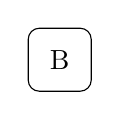
\begin{tikzpicture}
        \node[rounded corners,draw=black,minimum size=0.8cm]{B};
    \end{tikzpicture}
    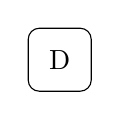
\begin{tikzpicture}
        \node[rounded corners,draw=black,minimum size=0.8cm]{D};
    \end{tikzpicture}
    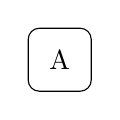
\begin{tikzpicture}
        \node[rounded corners,draw=black,minimum size=0.8cm]{A};
    \end{tikzpicture}
    };  

     \node[text width=3cm] at (-3,-10) 
    {Hit on B};

    \node[rounded corners,draw=black,minimum size=2cm, below left=1 cm of d] (f) at (2.2,-11)  { 
    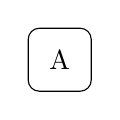
\begin{tikzpicture}
        \node[rounded corners,draw=black,minimum size=0.8cm]{A};
    \end{tikzpicture}
    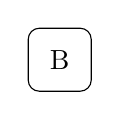
\begin{tikzpicture}
        \node[rounded corners,draw=black,minimum size=0.8cm]{B};
    \end{tikzpicture}
    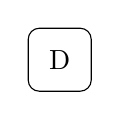
\begin{tikzpicture}
        \node[rounded corners,draw=black,minimum size=0.8cm]{D};
    \end{tikzpicture}
    };  

     \node[text width=3cm] at (-3,-12.5) 
    {Hit on D};

    \node[rounded corners,draw=black,minimum size=2cm, below left=1 cm of d] (g) at (2.2,-13.5)  { 
    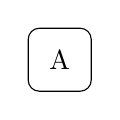
\begin{tikzpicture}
        \node[rounded corners,draw=black,minimum size=0.8cm]{A};
    \end{tikzpicture}
    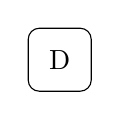
\begin{tikzpicture}
        \node[rounded corners,draw=black,minimum size=0.8cm]{D};
    \end{tikzpicture}
    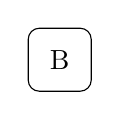
\begin{tikzpicture}
        \node[rounded corners,draw=black,minimum size=0.8cm]{B};
    \end{tikzpicture}
    };  

     \node[text width=3cm] at (-3,-15) 
    {Hit on A};

    \draw[thick,->] (a) -- (b);
    \draw[thick,->](b) -- (c);  
    \draw[thick,->](c) -- (d);  
    \draw[thick,->](d) -- (e);  
    \draw[thick,->](e) -- (f);  
    \draw[thick,->](f) -- (g);  
\end{tikzpicture}
\end{figure}

\section{Measuring algorithm Performance}
Given these algorithms, one may consider looking at a set of traces to see which algorithm performs better. Let's do this in the paging model with the two traces in Figures 3.2 and 3.3.

On the trace in Figure 3.2, LRU ends up missing less than MRU. As discussed before, we aim to minimize the total number of misses in a cache as they cause the system to slow down. So given this trace and this cache size, we want to choose LRU to maximize performance.

On the trace in Figure 3.3, MRU ends up missing less than LRU. So given this trace and this cache size, we want to choose MRU to maximize performance.

\begin{figure}[h]
    
    \centering
    \caption{How MRU performs against LRU given the trace: A, B, C, D, C}
    \label{fig:my_label}
    \scalebox{.85}{
\begin{tikzpicture} 
    \node[rounded corners,draw=black,label=above:MRU, minimum size=2cm] (a) at (0,0)  {
    \begin{tikzpicture}
        \node[rounded corners,draw=black,minimum size=0.8cm]{A};
    \end{tikzpicture}
    
\begin{tikzpicture}
        \node[rounded corners,draw=black,minimum size=0.8cm]{};
    \end{tikzpicture}
    
\begin{tikzpicture}
        \node[rounded corners,draw=black,minimum size=0.8cm]{};
    \end{tikzpicture}
    };
    \node[text width=3cm] at (-3, 0) 
    {Miss on A, A added to cache};

    
    \node[rounded corners,draw=black,minimum size=2cm] (b) at (0,-2.5)  {   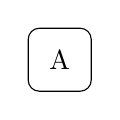
\begin{tikzpicture}
        \node[rounded corners,draw=black,minimum size=0.8cm]{A};
    \end{tikzpicture}
    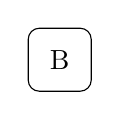
\begin{tikzpicture}
        \node[rounded corners,draw=black,minimum size=0.8cm]{B};
    \end{tikzpicture}
    
\begin{tikzpicture}
        \node[rounded corners,draw=black,minimum size=0.8cm]{};
    \end{tikzpicture}
    };
     \node[text width=3cm] at (-3,-2.5) 
    {Miss on B, B added to cache};
    
    \node[rounded corners,draw=black,minimum size=2cm] (c) at (0,-5)  {   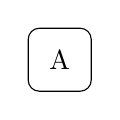
\begin{tikzpicture}
        \node[rounded corners,draw=black,minimum size=0.8cm]{A};
    \end{tikzpicture}
    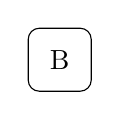
\begin{tikzpicture}
        \node[rounded corners,draw=black,minimum size=0.8cm]{B};
    \end{tikzpicture}
    \begin{tikzpicture}
        \node[rounded corners,draw=black,minimum size=0.8cm]{C};
    \end{tikzpicture}
    };

    \node[text width=3cm] at (-3,-5) 
    {Miss on C, C added to cache};
      
    \node[rounded corners,draw=black,minimum size=2cm] (d) at (0,-7.5)  {   \begin{tikzpicture}
        \node[rounded corners,draw=black,minimum size=0.8cm]{A};
    \end{tikzpicture}
    \begin{tikzpicture}
        \node[rounded corners,draw=black,minimum size=0.8cm]{B};
    \end{tikzpicture}
    \begin{tikzpicture}
        \node[rounded corners,draw=black,minimum size=0.8cm]{D};
    \end{tikzpicture}
    };

     \node[text width=3cm] at (-3,-7.5) 
    {Miss on D, D added to cache, evict C since MRU};
    
    \node[rounded corners,draw=black,minimum size=2cm, below left=1 cm of d] (e) at (2.2,-8.4)  { 
    \begin{tikzpicture}
        \node[rounded corners,draw=black,minimum size=0.8cm]{A};
    \end{tikzpicture}
    \begin{tikzpicture}
        \node[rounded corners,draw=black,minimum size=0.8cm]{B};
    \end{tikzpicture}
    \begin{tikzpicture}
        \node[rounded corners,draw=black,minimum size=0.8cm]{C};
    \end{tikzpicture}
    };  

     \node[text width=2.5cm] at (-2.5,-9.8) 
    {Miss on C, evict D since MRU};
















    %LRU
    \node[rounded corners,draw=black,label=above:LRU, minimum size=2cm] (i) at (6,0)  {
    \begin{tikzpicture}
        \node[rounded corners,draw=black,minimum size=0.8cm]{A};
    \end{tikzpicture}
    \begin{tikzpicture}
        \node[rounded corners,draw=black,minimum size=0.8cm]{};
    \end{tikzpicture}
    \begin{tikzpicture}
        \node[rounded corners,draw=black,minimum size=0.8cm]{};
    \end{tikzpicture}
    };
    \node[text width=3cm] at (10,0) 
    {Miss on A, A added to cache};
    \node[text width=3cm] at (4,0) 
    {\Huge A};

    
    \node[rounded corners,draw=black,minimum size=2cm] (j) at (6,-2.5)  {   \begin{tikzpicture}
        \node[rounded corners,draw=black,minimum size=0.8cm]{A};
    \end{tikzpicture}
    \begin{tikzpicture}
        \node[rounded corners,draw=black,minimum size=0.8cm]{B};
    \end{tikzpicture}
    \begin{tikzpicture}
        \node[rounded corners,draw=black,minimum size=0.8cm]{};
    \end{tikzpicture}
    };
    \node[text width=3cm] at (10,-2.4) 
    {Miss on B, B added to cache};
    \node[text width=3cm] at (4,-2.4) 
    {\Huge B};
    
    \node[rounded corners,draw=black,minimum size=2cm] (k) at (6,-5)  {   \begin{tikzpicture}
        \node[rounded corners,draw=black,minimum size=0.8cm]{A};
    \end{tikzpicture}
    \begin{tikzpicture}
        \node[rounded corners,draw=black,minimum size=0.8cm]{B};
    \end{tikzpicture}
    \begin{tikzpicture}
        \node[rounded corners,draw=black,minimum size=0.8cm]{C};
    \end{tikzpicture}
    };
    \node[text width=3cm] at (10,-4.8) 
    {Miss on C, C added to cache};
    \node[text width=3cm] at (4,-4.8) 
    {\Huge C};
    
      
    \node[rounded corners,draw=black,minimum size=2cm] (l) at (6,-7.5)  {   \begin{tikzpicture}
        \node[rounded corners,draw=black,minimum size=0.8cm]{D};
    \end{tikzpicture}
    \begin{tikzpicture}
        \node[rounded corners,draw=black,minimum size=0.8cm]{B};
    \end{tikzpicture}
    \begin{tikzpicture}
        \node[rounded corners,draw=black,minimum size=0.8cm]{C};
    \end{tikzpicture}
    };
     \node[text width=3cm] at (10,-7.4) 
    {Miss on D, D added to cache, Evict A since LRU};
    \node[text width=3cm] at (4,-7.4) 
    {\Huge D};

    
    \node[rounded corners,draw=black,minimum size=2cm, below left=1 cm of l] (m) at (8.2,-8.4)  { 
    \begin{tikzpicture}
        \node[rounded corners,draw=black,minimum size=0.8cm]{D};
    \end{tikzpicture}
    \begin{tikzpicture}
        \node[rounded corners,draw=black,minimum size=0.8cm]{A};
    \end{tikzpicture}
    \begin{tikzpicture}
        \node[rounded corners,draw=black,minimum size=0.8cm]{C};
    \end{tikzpicture}
    };  
    \node[text width=3cm] at (10,-10) 
    {Hit on C};
    \node[text width=3cm] at (4,-10) 
    {\Huge C};


    \draw[thick,->] (a) -- (b);
    \draw[thick,->](b) -- (c);  
    \draw[thick,->](c) -- (d);  
    \draw[thick,->](d) -- (e);  

    
    \draw[thick,->] (i) -- (j);
    \draw[thick,->](j) -- (k);  
    \draw[thick,->](k) -- (l);  
    \draw[thick,->](l) -- (m);  
\end{tikzpicture}
}
\end{figure}
\hfill \break
\hfill \break
\hfill \break
\hfill \break
\hfill \break
\hfill \break
\hfill \break
\hfill \break

\begin{figure}[H]
    \centering
    \caption{How MRU performs against LRU given the trace: A, B, C, D, A}
    \label{fig:my_label}
\scalebox{.85}{
    \begin{tikzpicture} 
    \node[rounded corners,draw=black,label=above:MRU, minimum size=2cm] (a) at (0,0)  {
    \begin{tikzpicture}
        \node[rounded corners,draw=black,minimum size=0.8cm]{A};
    \end{tikzpicture}
    \begin{tikzpicture}
        \node[rounded corners,draw=black,minimum size=0.8cm]{};
    \end{tikzpicture}
    \begin{tikzpicture}
        \node[rounded corners,draw=black,minimum size=0.8cm]{};
    \end{tikzpicture}
    };
    \node[text width=3cm] at (-3, 0) 
    {Miss on A, A added to cache};

    
    \node[rounded corners,draw=black,minimum size=2cm] (b) at (0,-2.5)  {   \begin{tikzpicture}
        \node[rounded corners,draw=black,minimum size=0.8cm]{A};
    \end{tikzpicture}
    \begin{tikzpicture}
        \node[rounded corners,draw=black,minimum size=0.8cm]{B};
    \end{tikzpicture}
    \begin{tikzpicture}
        \node[rounded corners,draw=black,minimum size=0.8cm]{};
    \end{tikzpicture}
    };
     \node[text width=3cm] at (-3,-2.5) 
    {Miss on B, B added to cache};
    
    \node[rounded corners,draw=black,minimum size=2cm] (c) at (0,-5)  {   \begin{tikzpicture}
        \node[rounded corners,draw=black,minimum size=0.8cm]{A};
    \end{tikzpicture}
    \begin{tikzpicture}
        \node[rounded corners,draw=black,minimum size=0.8cm]{B};
    \end{tikzpicture}
    \begin{tikzpicture}
        \node[rounded corners,draw=black,minimum size=0.8cm]{C};
    \end{tikzpicture}
    };

    \node[text width=3cm] at (-3,-5) 
    {Miss on C, C added to cache};
      
    \node[rounded corners,draw=black,minimum size=2cm] (d) at (0,-7.5)  {   \begin{tikzpicture}
        \node[rounded corners,draw=black,minimum size=0.8cm]{A};
    \end{tikzpicture}
    \begin{tikzpicture}
        \node[rounded corners,draw=black,minimum size=0.8cm]{B};
    \end{tikzpicture}
    \begin{tikzpicture}
        \node[rounded corners,draw=black,minimum size=0.8cm]{D};
    \end{tikzpicture}
    };

     \node[text width=3cm] at (-3,-7.5) 
    {Miss on D, add D to cache, evict C since MRU};
    
    \node[rounded corners,draw=black,minimum size=2cm, below left=1 cm of d] (e) at (2.2,-8.4)  { 
    \begin{tikzpicture}
        \node[rounded corners,draw=black,minimum size=0.8cm]{A};
    \end{tikzpicture}
    \begin{tikzpicture}
        \node[rounded corners,draw=black,minimum size=0.8cm]{B};
    \end{tikzpicture}
    \begin{tikzpicture}
        \node[rounded corners,draw=black,minimum size=0.8cm]{C};
    \end{tikzpicture}
    };  

     \node[text width=2.5cm] at (-2.5,-9.8) 
    {Hit on A};
















    %LRU
    \node[rounded corners,draw=black,label=above:LRU, minimum size=2cm] (i) at (6,0)  {
    \begin{tikzpicture}
        \node[rounded corners,draw=black,minimum size=0.8cm]{A};
    \end{tikzpicture}
    \begin{tikzpicture}
        \node[rounded corners,draw=black,minimum size=0.8cm]{};
    \end{tikzpicture}
    \begin{tikzpicture}
        \node[rounded corners,draw=black,minimum size=0.8cm]{};
    \end{tikzpicture}
    };
    \node[text width=3cm] at (10,0) 
    {Miss on A, A added to cache};
    \node[text width=3cm] at (4,0) 
    {\Huge A};

    
    \node[rounded corners,draw=black,minimum size=2cm] (j) at (6,-2.5)  {   \begin{tikzpicture}
        \node[rounded corners,draw=black,minimum size=0.8cm]{A};
    \end{tikzpicture}
    \begin{tikzpicture}
        \node[rounded corners,draw=black,minimum size=0.8cm]{B};
    \end{tikzpicture}
    \begin{tikzpicture}
        \node[rounded corners,draw=black,minimum size=0.8cm]{};
    \end{tikzpicture}
    };
    \node[text width=3cm] at (10,-2.4) 
    {Miss on B, B added to cache};
    \node[text width=3cm] at (4,-2.4) 
    {\Huge B};
    
    \node[rounded corners,draw=black,minimum size=2cm] (k) at (6,-5)  {   \begin{tikzpicture}
        \node[rounded corners,draw=black,minimum size=0.8cm]{A};
    \end{tikzpicture}
    \begin{tikzpicture}
        \node[rounded corners,draw=black,minimum size=0.8cm]{B};
    \end{tikzpicture}
    \begin{tikzpicture}
        \node[rounded corners,draw=black,minimum size=0.8cm]{C};
    \end{tikzpicture}
    };
    \node[text width=3cm] at (10,-4.8) 
    {Miss on C, C added to cache};
    \node[text width=3cm] at (4,-4.8) 
    {\Huge C};
    
      
    \node[rounded corners,draw=black,minimum size=2cm] (l) at (6,-7.5)  {   \begin{tikzpicture}
        \node[rounded corners,draw=black,minimum size=0.8cm]{D};
    \end{tikzpicture}
    \begin{tikzpicture}
        \node[rounded corners,draw=black,minimum size=0.8cm]{B};
    \end{tikzpicture}
    \begin{tikzpicture}
        \node[rounded corners,draw=black,minimum size=0.8cm]{C};
    \end{tikzpicture}
    };
     \node[text width=3cm] at (10,-7.4) 
    {Miss on D, D added to cache, Evict A since LRU};
    \node[text width=3cm] at (4,-7.4) 
    {\Huge D};

    
    \node[rounded corners,draw=black,minimum size=2cm, below left=1 cm of l] (m) at (8.2,-8.4)  { 
    \begin{tikzpicture}
        \node[rounded corners,draw=black,minimum size=0.8cm]{D};
    \end{tikzpicture}
    \begin{tikzpicture}
        \node[rounded corners,draw=black,minimum size=0.8cm]{A};
    \end{tikzpicture}
    \begin{tikzpicture}
        \node[rounded corners,draw=black,minimum size=0.8cm]{C};
    \end{tikzpicture}
    };  
    \node[text width=3cm] at (10,-10) 
    {Miss on A, A added to cache, evict B since LRU};
    \node[text width=3cm] at (4,-10) 
    {\Huge A};


    \draw[thick,->] (a) -- (b);
    \draw[thick,->](b) -- (c);  
    \draw[thick,->](c) -- (d);  
    \draw[thick,->](d) -- (e);  

    
    \draw[thick,->] (i) -- (j);
    \draw[thick,->](j) -- (k);  
    \draw[thick,->](k) -- (l);  
    \draw[thick,->](l) -- (m);  
\end{tikzpicture}
}
\end{figure}

Does the fact that these algorithms perform differently on these traces mean that comparison of algorithms on traces is not a useful metric? No. These traces are what are called adversarial traces, meaning that they are specifically made to make an algorithm perform as badly as it possibly can. So trace 1 in Figure 3.2 is made specifically to perform poorly with MRU. If this trace were to be repeated, MRU would begin to miss every item. The same is true of LRU in the trace from Figure 3.3.

These adversarial traces pose a challenge, as there will almost always be a way to structure a trace so that any algorithm A has maximal misses. Even looking at how they perform over a large set of traces does not give much insight, as there are infinitely many traces that can be tested. So instead of looking at comparing these algorithms on any specific trace or set of traces, we instead seek to look to create a more even playing field for these algorithms' performance to be judged.
\hfill \break
\hfill \break
\hfill \break
\hfill \break
\hfill \break


\section{Competitive Ratios}
Competitive ratios are the ways that we can bound the performance of an algorithm more fairly than by testing directly on traces. These ratios are theoretical, meaning they are a good measurement of how algorithms perform in the abstract.

Now to find these competitive ratios, we compare algorithm A to algorithm B. Specifically, given $\sigma$ so that algorithm B performs with minimum misses on the trace. Then we compare the number of misses they both have, giving us that competitive ratio of $\frac{misses(A)}{misses(B)}$. The question then becomes: how does one decide this B so that it has minimal misses? This is done through the use of an optimal algorithm.

\subsection{Optimal Algorithms}
Offline algorithms are a class of algorithms used in computer science that operate using information about an entire trace to make decisions rather than processing data as it arrives a request at a time. Optimal algorithms are then required to be offline to minimize misses as they need to see the entire trace to make eviction decisions. The algorithms we have discussed so far have all been Online algorithms, meaning they process items 1 request at a time and can only make decisions based on current and past requests. 

This distinction between these online and offline algorithms means that optimal algorithms have the entirety of the input data available in advance, and can take as much time and memory as needed to produce the output with the least number of misses in the paging model. This trait means we can then use them to bind how an algorithm performs as they always perform with these minimal number of misses. 

OPT works in the paging model by, when needing to evict an item, finding the item that is furthest in the future. This is because the item furthest in the future has the

Figure 3.4 is an example of how OPT uses its knowledge of the entire trace to make minimal misses when compared to LRU. In this trace, OPT only misses on the first instance of an item and manages to hit on all others, while LRU manages to miss on the last A and B as well as all items OPT misses. This is because OPT can process the entire trace before making any decisions and can then keep misses minimal. 

Now that there is this OPT algorithm that we can compare other algorithms to, we want to see what the best performance case is for algorithm A when compared to OPT. We want to do this because OPT always performs the best any algorithm can on a trace. This means that when compared to OPT, all other algorithms are put onto the same playing field.


\hfill \break
\hfill \break
\hfill \break
\hfill \break
\hfill \break
\hfill \break
\hfill \break
\hfill \break
\hfill \break
\hfill \break


\begin{figure}[H]
    \centering
    \caption{How OPT performs when compared to an online algorithm LRU given the trace: A, B, C, D, A, B, C, C}
    \label{fig:my_label}
\begin{tikzpicture} 
    \node[rounded corners,draw=black,label=above:OPT, minimum size=2cm] (a) at (0,0)  {
    \begin{tikzpicture}
        \node[rounded corners,draw=black,minimum size=0.8cm]{A};
    \end{tikzpicture}
    \begin{tikzpicture}
        \node[rounded corners,draw=black,minimum size=0.8cm]{};
    \end{tikzpicture}
    \begin{tikzpicture}
        \node[rounded corners,draw=black,minimum size=0.8cm]{};
    \end{tikzpicture}
    };
    \node[text width=3cm] at (-3, 0) 
    {Miss on A, A added to cache};

    
    \node[rounded corners,draw=black,minimum size=2cm] (b) at (0,-2.5)  {   \begin{tikzpicture}
        \node[rounded corners,draw=black,minimum size=0.8cm]{A};
    \end{tikzpicture}
    \begin{tikzpicture}
        \node[rounded corners,draw=black,minimum size=0.8cm]{B};
    \end{tikzpicture}
    \begin{tikzpicture}
        \node[rounded corners,draw=black,minimum size=0.8cm]{};
    \end{tikzpicture}
    };
     \node[text width=3cm] at (-3,-2.5) 
    {Miss on B, B added to cache};
    
    \node[rounded corners,draw=black,minimum size=2cm] (c) at (0,-5)  {   \begin{tikzpicture}
        \node[rounded corners,draw=black,minimum size=0.8cm]{A};
    \end{tikzpicture}
    \begin{tikzpicture}
        \node[rounded corners,draw=black,minimum size=0.8cm]{B};
    \end{tikzpicture}
    \begin{tikzpicture}
        \node[rounded corners,draw=black,minimum size=0.8cm]{C};
    \end{tikzpicture}
    };

    \node[text width=3cm] at (-3,-5) 
    {Miss on C, C added to cache};
      
    \node[rounded corners,draw=black,minimum size=2cm] (d) at (0,-7.5)  {   \begin{tikzpicture}
        \node[rounded corners,draw=black,minimum size=0.8cm]{A};
    \end{tikzpicture}
    \begin{tikzpicture}
        \node[rounded corners,draw=black,minimum size=0.8cm]{B};
    \end{tikzpicture}
    \begin{tikzpicture}
        \node[rounded corners,draw=black,minimum size=0.8cm]{D};
    \end{tikzpicture}
    };

     \node[text width=3cm] at (-3,-7.5) 
    {Miss on D, D added to cache, evict C since FITF};
    
    \node[rounded corners,draw=black,minimum size=2cm, below left=1 cm of d] (e) at (2.2,-8.4)  { 
    \begin{tikzpicture}
        \node[rounded corners,draw=black,minimum size=0.8cm]{A};
    \end{tikzpicture}
    \begin{tikzpicture}
        \node[rounded corners,draw=black,minimum size=0.8cm]{B};
    \end{tikzpicture}
    \begin{tikzpicture}
        \node[rounded corners,draw=black,minimum size=0.8cm]{D};
    \end{tikzpicture}
    };  

     \node[text width=3cm] at (-2.5,-9.8) 
    {Hit on A};
    
    \node[rounded corners,draw=black,minimum size=2cm,below left=1 cm of e] (f) at (2.2,-10.8)  { 
    \begin{tikzpicture}
        \node[rounded corners,draw=black,minimum size=0.8cm]{A};
    \end{tikzpicture}
    \begin{tikzpicture}
        \node[rounded corners,draw=black,minimum size=0.8cm]{B};
    \end{tikzpicture}
    \begin{tikzpicture}
        \node[rounded corners,draw=black,minimum size=0.8cm]{D};
    \end{tikzpicture}
    };  

     \node[text width=3cm] at (-2.5,-12.2) 
    {Hit on B};

    
    \node[rounded corners,draw=black,minimum size=2cm, below left=1 cm of f] (g) at (2.2,-13.4)  { 
    \begin{tikzpicture}
        \node[rounded corners,draw=black,minimum size=0.8cm]{A};
    \end{tikzpicture}
    \begin{tikzpicture}
        \node[rounded corners,draw=black,minimum size=0.8cm]{B};
    \end{tikzpicture}
    \begin{tikzpicture}
        \node[rounded corners,draw=black,minimum size=0.8cm]{D};
    \end{tikzpicture}
    };  

     \node[text width=3cm] at (-3,-14.7) 
    {Miss on C, evict D};
    
    \node[rounded corners,draw=black,minimum size=2cm, below left=1 cm of g] (h) at (2.2,-15.6)  { 
    \begin{tikzpicture}
        \node[rounded corners,draw=black,minimum size=0.8cm]{A};
    \end{tikzpicture}
    \begin{tikzpicture}
        \node[rounded corners,draw=black,minimum size=0.8cm]{B};
    \end{tikzpicture}
    \begin{tikzpicture}
        \node[rounded corners,draw=black,minimum size=0.8cm]{C};
    \end{tikzpicture}
    }; 
    \node[text width=3cm] at (-2.5,-17.3) 
    {Hit on C};






















    %LRU
    \node[rounded corners,draw=black,label=above:LRU, minimum size=2cm] (i) at (6,0)  {
    \begin{tikzpicture}
        \node[rounded corners,draw=black,minimum size=0.8cm]{A};
    \end{tikzpicture}
    \begin{tikzpicture}
        \node[rounded corners,draw=black,minimum size=0.8cm]{};
    \end{tikzpicture}
    \begin{tikzpicture}
        \node[rounded corners,draw=black,minimum size=0.8cm]{};
    \end{tikzpicture}
    };
    \node[text width=3cm] at (10,0) 
    {Miss on A, A added to cache};
    \node[text width=3cm] at (4,0) 
    {\Huge A};

    
    \node[rounded corners,draw=black,minimum size=2cm] (j) at (6,-2.5)  {   \begin{tikzpicture}
        \node[rounded corners,draw=black,minimum size=0.8cm]{A};
    \end{tikzpicture}
    \begin{tikzpicture}
        \node[rounded corners,draw=black,minimum size=0.8cm]{B};
    \end{tikzpicture}
    \begin{tikzpicture}
        \node[rounded corners,draw=black,minimum size=0.8cm]{};
    \end{tikzpicture}
    };
    \node[text width=3cm] at (10,-2.4) 
    {Miss on B, B added to cache};
    \node[text width=3cm] at (4,-2.4) 
    {\Huge B};
    
    \node[rounded corners,draw=black,minimum size=2cm] (k) at (6,-5)  {   \begin{tikzpicture}
        \node[rounded corners,draw=black,minimum size=0.8cm]{A};
    \end{tikzpicture}
    \begin{tikzpicture}
        \node[rounded corners,draw=black,minimum size=0.8cm]{B};
    \end{tikzpicture}
    \begin{tikzpicture}
        \node[rounded corners,draw=black,minimum size=0.8cm]{C};
    \end{tikzpicture}
    };
    \node[text width=3cm] at (10,-4.8) 
    {Miss on C, C added to cache};
    \node[text width=3cm] at (4,-4.8) 
    {\Huge C};
    
      
    \node[rounded corners,draw=black,minimum size=2cm] (l) at (6,-7.5)  {   \begin{tikzpicture}
        \node[rounded corners,draw=black,minimum size=0.8cm]{D};
    \end{tikzpicture}
    \begin{tikzpicture}
        \node[rounded corners,draw=black,minimum size=0.8cm]{B};
    \end{tikzpicture}
    \begin{tikzpicture}
        \node[rounded corners,draw=black,minimum size=0.8cm]{C};
    \end{tikzpicture}
    };
     \node[text width=3cm] at (10,-7.4) 
    {Miss on D, Evict A as LRU};
    \node[text width=3cm] at (4,-7.4) 
    {\Huge D};

    
    \node[rounded corners,draw=black,minimum size=2cm, below left=1 cm of l] (m) at (8.2,-8.4)  { 
    \begin{tikzpicture}
        \node[rounded corners,draw=black,minimum size=0.8cm]{D};
    \end{tikzpicture}
    \begin{tikzpicture}
        \node[rounded corners,draw=black,minimum size=0.8cm]{A};
    \end{tikzpicture}
    \begin{tikzpicture}
        \node[rounded corners,draw=black,minimum size=0.8cm]{C};
    \end{tikzpicture}
    };  
    \node[text width=3cm] at (10,-10) 
    {Miss on A, Evict B since LRU};
    \node[text width=3cm] at (4,-10) 
    {\Huge A};

    
    \node[rounded corners,draw=black,minimum size=2cm,below left=1 cm of m] (n) at (8.2,-10.8)  { 
    \begin{tikzpicture}
        \node[rounded corners,draw=black,minimum size=0.8cm]{D};
    \end{tikzpicture}
    \begin{tikzpicture}
        \node[rounded corners,draw=black,minimum size=0.8cm]{A};
    \end{tikzpicture}
    \begin{tikzpicture}
        \node[rounded corners,draw=black,minimum size=0.8cm]{B};
    \end{tikzpicture}
    };  
     \node[text width=3cm] at (10,-12.3) 
    {Miss on B, Evict C since LRU};
    \node[text width=3cm] at (4,-12.3) 
    {\Huge B};

    
    \node[rounded corners,draw=black,minimum size=2cm, below left=1 cm of n] (o) at (8.2,-13.4)  { 
    \begin{tikzpicture}
        \node[rounded corners,draw=black,minimum size=0.8cm]{C};
    \end{tikzpicture}
    \begin{tikzpicture}
        \node[rounded corners,draw=black,minimum size=0.8cm]{A};
    \end{tikzpicture}
    \begin{tikzpicture}
        \node[rounded corners,draw=black,minimum size=0.8cm]{B};
    \end{tikzpicture}
    };  
    \node[text width=3cm] at (10,-14.8) 
    {Miss on C, evict B};
    \node[text width=3cm] at (4,-14.8) 
    {\Huge C};
    
    
    \node[rounded corners,draw=black,minimum size=2cm, below left=1 cm of o] (p) at (8.2,-15.6)  { 
    \begin{tikzpicture}
        \node[rounded corners,draw=black,minimum size=0.8cm]{C};
    \end{tikzpicture}
    \begin{tikzpicture}
        \node[rounded corners,draw=black,minimum size=0.8cm]{A};
    \end{tikzpicture}
    \begin{tikzpicture}
        \node[rounded corners,draw=black,minimum size=0.8cm]{B};
    \end{tikzpicture}
    };  
    \node[text width=3cm] at (10,-17.3) 
    {Hit on C};
    \node[text width=3cm] at (4,-17.3) 
    {\Huge C};

    \draw[thick,->] (a) -- (b);
    \draw[thick,->](b) -- (c);  
    \draw[thick,->](c) -- (d);  
    \draw[thick,->](d) -- (e);  
    \draw[thick,->] (e) -- (f);
    \draw[thick,->](f) -- (g);  
    \draw[thick,->](g) -- (h);
    
    \draw[thick,->] (i) -- (j);
    \draw[thick,->](j) -- (k);  
    \draw[thick,->](k) -- (l);  
    \draw[thick,->](l) -- (m);  
    \draw[thick,->] (m) -- (n);
    \draw[thick,->](n) -- (o);  
    \draw[thick,->](o) -- (p);
        
\end{tikzpicture}
\end{figure}

\subsection{Competitive Lower Bounds}
The lower competitive bound refers to the minimum ratio of misses any algorithm A can have when compared to OPT.

The minimum competitive bound for algorithms was first established by Sleator and Tarjan in their paper "Amortized efficiency of list update and paging rules" in 1985. They proved that the lower competitive bound of all deterministic algorithms when compared to OPT is $\frac{k}{k-h+1}$ \cite{sleator1985amortized}. Where $h$ is the size of OPTs cache and $k$ is the size of the algorithms cache.

This result from Sleator and Tarjan shows that no algorithm processing a trace one request at a time can achieve a competitive ratio better than $\frac{k}{k-h+1}$, regardless of its design or implementation. As a result, much of the research in caching algorithms has focused on developing algorithms that can achieve competitive ratios that are close to or equal to this lower bound.

This alone doesn't mean that algorithms always perform this poorly when compared to OPT as it is just a lower bound for how well it can do. Instead, when looking to see how an algorithm performs, we also look to see what its upper bounds are.



\section{Upper Bounds}
The upper competitive bound refers to the maximum competitive ratio that any algorithm can achieve relative to OPT, and unlike competitive lower bounds, there is no maximum upper bound. This means that there is no maximum cost ratio that an algorithm can pay when compared to OPT.

This means that algorithms are designed to have upper bounds to be as close to the minimal lower bound $\frac{k}{k-h+1}$ as possible. If an algorithm achieves this upper bound, it would mean that its bounded competitive ratio is $\frac{k}{k-h+1}$. For an algorithm to have these matching bounds, it would mean that it performs as well as any algorithm can when compared to OPT.

LRU was shown in \cite{sleator1985amortized} to have these matching lower and upper bounds in the paging model. This means that LRU performs competitively to the minimum bounds of online caching algorithms in any circumstance in the paging model.
MRU was then shown \cite{agrawal2007worst} to have no maximum upper bound, this means that while MRU may have the same lower bound as LRU, it is possible to pay arbitrarily high cost when compared to OPT. So while LRU always will perform within this $\frac{k}{k-h+1}$ bound, MRU can reach this bound but could pay a much higher ratio.


\hfill \break
\hfill \break
\hfill \break


\section{Landlord}
The landlord algorithm was just one of a set of algorithms that Neal E. Young proposed in \cite{young1994k}. Landlord was created by Young to generalize LRU to the general model as it was limited to the paging model at the time. 

\makeatletter
\def\BState{\State\hskip-\ALG@thistlm}
\makeatother
\algnewcommand\algorithmicforeach{\textbf{for each}}
\algdef{S}[FOR]{ForEach}[1]{\algorithmicforeach\ #1\ \algorithmicdo}




    \begin{algorithm}
\caption{Landlord}\label{euclid}
    \begin{algorithmic}[1]
    \BState \emph{loop}:
        \State $\textit{Item} \gets \text{nextItem in trace}$
        \If {$\textit{Item} \text{ not in Cache}$}
            \While{$\text{Cache can't contain Item}$}
                \State $x \gets y\in cache \text{ with } min(\frac{cost(y)}{size(y)})$
                    \State $\Delta \gets \frac{credit(x)}{size(x)}$
                    \ForEach {$f \in cache $}
                        \State $credit(f) \gets credit(f) - \Delta \times size(f)$
                    \EndFor
                    \State $\exists f, credit(f)=0,\text{ Evict(f)} $        \EndWhile
            \State $credit(Item) \gets cost(Item)$
        \Else 
         \State $credit(i) \gets \text{value between current credit and cost}$
        \EndIf
    \end{algorithmic}
\end{algorithm}




As can be seen in this pseudo code, Landlord gives each item a credit C when it enters the cache from memory. This credit C is always positive as it is an estimation of how much you want this specific item in a cache.

When a replacement decision is made in Landlord, the items with 0 credit value are evicted. As requests get processed, the credit of all items in the cache gets reduced by a function of the lowest priority item's cost and size and the size of the item itself.

An important thing to note about Landlord is that if an item is already in the cache and is accessed again, its credit is reset to some number between an item's current credit and its max credit. This then allows items that are in the cache and accessed frequently to always have more credit than those in the cache that is accessed infrequently. This structure of credit renewal allows the algorithm to take advantage of the temporal locality of accesses.

Figure 3.5 shows how Landlord functions on an example trace and explains why it makes the evictions it does.


\begin{figure}[h]
    \centering
    \caption{Landlord's Performance on a trace}
    \label{fig:my_label}
Given cache size 3 and the trace: A,B,C,D,B,C,C,B with item costs 40,4,8,2 and size 1
\begin{tikzpicture}
\node[rounded corners, draw=black,label=above:Priorities, minimum width=5 cm](pri1) at (-8,0){
\begin{tikzpicture}
\node[rounded corners, draw=black, minimum width = 1cm](he){
a $=$ 40
};
\end{tikzpicture}
};
\node[rounded corners, text width = 4cm, left = 0 cm of pri1]{
Item a is given its cost as priority since space in cache
};

\node[rounded corners, draw=black, minimum width=5 cm](pri2) at (-8,-2.5){
\begin{tikzpicture}
\node[rounded corners, draw=black, minimum width = 1cm](he1){
a $=$ 36
};
\node[rounded corners, draw=black, minimum width = 1cm, left = .3cm of he1](he2){
b $=$ 4
};
\end{tikzpicture}

};
\node[rounded corners, text width = 4cm, left = 0 cm of pri2]{
Item b is given its cost as priority since space in cache, decrease A
};


\node[rounded corners, draw=black, minimum width=5 cm](pri3) at (-8,-5.2){
\begin{tikzpicture}
\node[rounded corners, draw=black, minimum width = 1cm](he1){
a $=$ 32
};
\node[rounded corners, draw=black, minimum width = 1cm, left = .3cm of he1](he2){
b $=$ 0
};
\node[rounded corners, draw=black, minimum width = 1cm, left = .3cm of he2](he3){
c $=$ 8
};
\end{tikzpicture}

};
\node[rounded corners, text width = 4cm, left = 0 cm of pri3]{
Item c is given its cost as priority since space in cache, decrease A and B
};

\node[rounded corners, draw=black, minimum width=5 cm](pri4) at (-8,-7.4){
\begin{tikzpicture}
\node[rounded corners, draw=black, minimum width = 1cm](he1){
d $=$ 2
};
\node[rounded corners, draw=black, minimum width = 1cm, left = .3cm of he1](he2){
a $=$ 30
};
\node[rounded corners, draw=black, minimum width = 1cm, left = .3cm of he2](he3){
c $=$ 4
};
\end{tikzpicture}


};
\node[rounded corners, text width = 4cm, left = 0 cm of pri4]{
no room for d, items in cache have priority decreased by $\Delta$ and B evicted
};

\node[rounded corners, draw=black, minimum width=5 cm](pri5) at (-8,-10){
\begin{tikzpicture}
\node[rounded corners, draw=black, minimum width = 1cm](he1){
b $=$ 4
};
\node[rounded corners, draw=black, minimum width = 1cm, left = .3cm of he1](he2){
a $=$ 26
};
\node[rounded corners, draw=black, minimum width = 1cm, left = .3cm of he2](he3){
c $=$ 0
};
\end{tikzpicture}

};

\node[rounded corners, text width = 4cm, left = 0 cm of pri5]{
B credit reset and others decreased by $\Delta$
};

\node[rounded corners, draw=black, minimum width=5 cm](pri6) at (-8,-12.3){
\begin{tikzpicture}
\node[rounded corners, draw=black, minimum width = 1cm, left = .3cm of he1](he2){
a $=$ 18
};
\node[rounded corners, draw=black, minimum width = 1cm, left = .3cm of he2](he3){
c $=$ 8
};
\end{tikzpicture}

};
\node[rounded corners, text width = 4cm, left = 0 cm of pri6]{
C credit reset and others decreased by $\Delta$
};


\node[rounded corners, draw=black, minimum width=5 cm](pri7) at (-8,-15){
\begin{tikzpicture}
\node[rounded corners, draw=black, minimum width = 1cm](he2){
a $=$ 10
};
\node[rounded corners, draw=black, minimum width = 1cm, left = .3cm of he2](he3){
c $=$ 8
};
\end{tikzpicture}

};
\node[rounded corners, text width = 4cm, left = 0 cm of pri7]{
C credit reset and others decreased by $\Delta$
};


\node[rounded corners, draw=black, minimum width=5 cm](pri8) at (-8,-17.2){
\begin{tikzpicture}
\node[rounded corners, draw=black, minimum width = 1cm](he1){
b $=$ 4
};
\node[rounded corners, draw=black, minimum width = 1cm, left = .3cm of he1](he2){
a $=$ 6
};
\node[rounded corners, draw=black, minimum width = 1cm, left = .3cm of he2](he3){
c $=$ 8
};
\end{tikzpicture}
};
\node[rounded corners, text width = 4cm, left = 0 cm of pri8]{
B credit reset and others decreased by $\Delta$
};
 
\end{tikzpicture}
   

\end{figure}


Landlord was shown in \cite{young1994k} to have both a lower and upper competitive ratio of $\frac{k}{k-h+1}$ in the general model. This means that Landlord can perform as well as any algorithm can when compared to OPT.
